% Model, chatbot, agent: the same function with more machinery around it.
% ---------------------------------------------------------------------------
% style.tex --- shared preamble for every figure in book/figures/tikz/
%
% One style for all figures: Latin Modern, thin black lines, a light grey
% fill, and one accent colour used only to mark what is untrusted or wrong.
% Build with scripts/build_figures.sh; see book/figures/README.md.
% ---------------------------------------------------------------------------
\documentclass[tikz,border=6pt]{standalone}
\usepackage[T1]{fontenc}
\usepackage{lmodern}
\usetikzlibrary{arrows.meta,positioning,shapes.geometric,calc,fit,backgrounds}

\hyphenpenalty=10000   % short lines in boxes: ragged, never hyphenated

\definecolor{lightgrey}{gray}{0.92}
\definecolor{accent}{HTML}{9B2D20}

\tikzset{
  every picture/.style={
    line width=0.6pt,
    font=\small,
    >={Stealth[length=5pt,width=4pt]},
    node distance=14pt and 24pt,
  },
  % shapes
  box/.style={draw, rectangle, inner xsep=8pt, inner ysep=5pt,
              minimum height=22pt, align=center},
  grey/.style={box, fill=lightgrey},
  rounded/.style={box, rounded corners=9pt},
  decision/.style={draw, diamond, aspect=2.4, inner sep=1.5pt, align=center},
  group/.style={draw, dashed, rounded corners=5pt, inner sep=7pt},
  % text
  tag/.style={font=\footnotesize, align=center, inner sep=2pt},
  note/.style={font=\footnotesize\itshape, align=center, inner sep=2pt},
  code/.style={font=\small\ttfamily},
  codetag/.style={font=\footnotesize\ttfamily, align=center, inner sep=2pt},
  title/.style={font=\small\scshape, align=center, inner sep=2pt},
  % lines
  arrow/.style={->},
  back/.style={->, dashed},
  thin/.style={line width=0.4pt, gray},
  % the one accent, for what is untrusted, wrong or missing
  bad/.style={accent},
  badbox/.style={box, draw=accent, text=accent},
}

\begin{document}
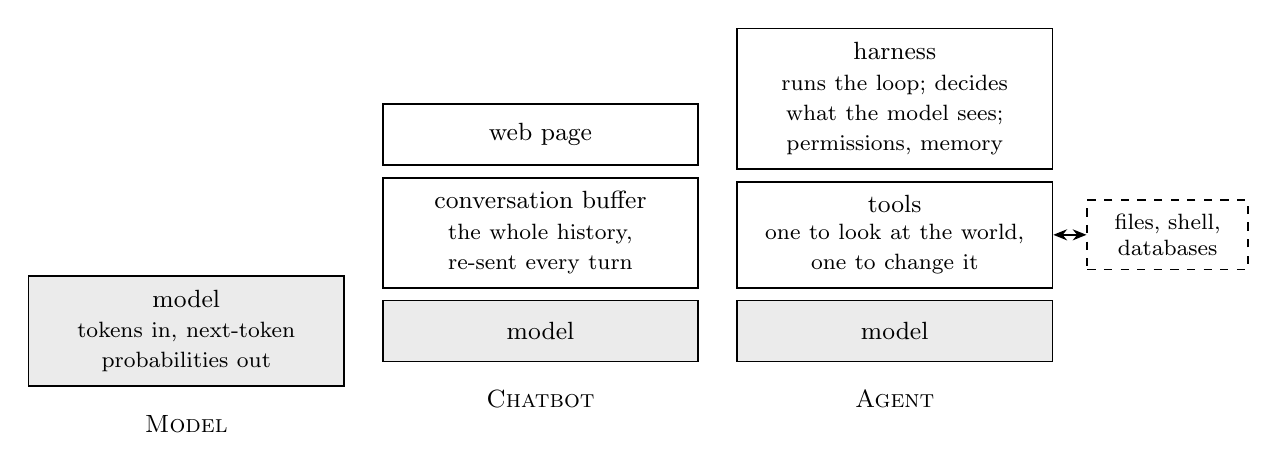
\begin{tikzpicture}[col/.style={text width=98pt, align=center}, node distance=4pt]
  % Model
  \node[grey, col] (m1) at (0,0) {model\\ \footnotesize tokens in, next-token probabilities out};
  \node[title, below=8pt of m1] {Model};
  % Chatbot
  \node[grey, col] (m2) at (128pt,0) {model};
  \node[box, col, above=of m2] (b2) {conversation buffer\\ \footnotesize the whole history, re-sent every turn};
  \node[box, col, above=of b2] (w2) {web page};
  \node[title, below=8pt of m2] {Chatbot};
  % Agent
  \node[grey, col] (m3) at (256pt,0) {model};
  \node[box, col, above=of m3] (t3) {tools\\ \footnotesize one to look at the world,\\ \footnotesize one to change it};
  \node[box, col, above=of t3] (h3) {harness\\ \footnotesize runs the loop; decides what the model sees; permissions, memory};
  \node[title, below=8pt of m3] {Agent};
  \node[box, dashed, right=12pt of t3, text width=42pt, align=center, font=\footnotesize] (world) {files, shell, databases};
  \draw[<->] (t3) -- (world);
\end{tikzpicture}
\end{document}
